
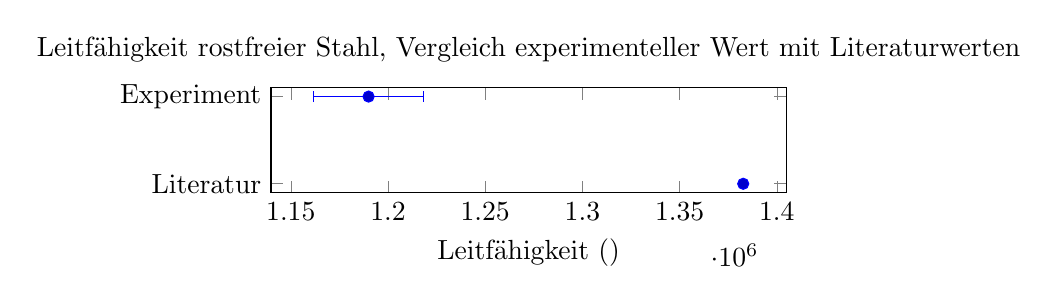
\begin{tikzpicture}
    \begin{axis}[
        try min ticks=2,
        width=.67\textwidth,
        height=.24\textwidth,
        title = {Leitf\"ahigkeit rostfreier Stahl, Vergleich experimenteller Wert mit Literaturwerten},
        xlabel = {Leitf\"ahigkeit ($\si{\ampere\per\volt\per\meter}$)},
        symbolic y coords = {Literatur,Experiment}
    ]
    \addplot+[
        only marks,error bars/.cd,
        x dir=both,x explicit,
        error bar style={line width=0.5pt},
        ]
    coordinates {%
        (1382711.1306243965,Literatur)
        (1190000.0,Experiment) +- (28108.0504482257,0)
    };
    \end{axis}
\end{tikzpicture}
\captionof{figure}{%
    Vergleich  der experimentell  bestimmten Leitf\"ahigkeit  f\"ur rostfreien
    Stahl  mit  einem  aus   Literaturwerten  bestimmten  Wert  (siehe  Anhang
    \ref{app:steel})%
    }
